% !Mode:: "TeX:UTF-8"
% Translator: Yujun Li 
\chapter{\glsentrytext{representation_learning}}
\label{chap:representation_learning}

% 517 head

在本章中,首先我们会讨论学习表示是什么意思,以及表示的概念如何有助于深度框架的设计。
我们探讨学习算法如何在不同任务中共享统计信息,包括使用\gls{unsupervised}任务中的信息来完成\gls{supervised}任务。
共享表示有助于处理多模式或多领域,或是将已学到的知识迁移到样本很少或没有、但任务表示依然存在的任务上。
最后,我们回过头探讨\gls{representation_learning}成功的原因,从\gls{distributed_representation}~\citep{Hinton-et-al-PDP1986}和深度表示的理论优势,最后会讲到\gls{DGP}潜在假设的更一般概念,特别是观测数据的基本成因。


很多信息处理任务可能非常容易,也可能非常困难,这取决于信息是如何表示的。
这是一个广泛适用于日常生活、计算机科学及\gls{ML}的基本原则。
例如,对于人而言,可以直接使用长除法计算$210$除以$6$。
但如果使用罗马数字表示,这个问题就没那么直接了。
大部分现代人在使用罗马数字计算\ENNAME{CCX}除以\ENNAME{VI}时,都会将其转化成阿拉伯数字,从而使用位值系统的长除法。
更具体地,我们可以使用合适或不合适的表示来量化不同操作的渐近运行时间。
例如,插入一个数字到有序表中的正确位置,如果该数列表示为链表,那么所需时间是$O(n)$;如果该列表表示为红黑树,那么只需要$O(\log n)$的时间。

% -- 517 --

在\gls{ML}中,到底是什么因素决定了一种表示比另一种表示更好呢?
一般而言,一个好的表示可以使后续的学习任务更容易。
选择什么表示通常取决于后续的学习任务。

% 518 head 


我们可以将\gls{supervised_learning}训练的\gls{feedforward_network}视为\gls{representation_learning}的一种形式。
具体地,网络的最后一层通常是\gls{linear_classifier},如\gls{softmax_chap15}回归分类器。
网络的其余部分学习出该分类器的表示。
监督学习训练模型,一般会使得模型的各个\gls{hidden_layer}(特别是接近顶层的\gls{hidden_layer})的表示能够更加容易地完成训练任务。
例如,输入特征线性不可分的类别可能在最后一个\gls{hidden_layer}变成线性\gls{separable}。
原则上,最后一层可以是另一种模型,如\gls{nearest_neighbor}分类器~\citep{SalakhutdinovR2007-small}。
倒数第二层的特征应该根据最后一层的类型学习不同的性质。
% 518 mid


\gls{feedforward_network}的\gls{supervised}训练并没有给\gls{learned}的中间特征明确强加任何条件。
其他的\gls{representation_learning}算法往往会以某种特定的方式明确设计表示。
例如,我们想要学习一种使得密度估计更容易的表示。
具有更多独立性的分布会更容易建模,因此,我们可以设计鼓励表示向量$\Vh$中元素之间相互独立的\gls{objective_function}。
就像\gls{supervised}网络,\gls{unsupervised}深度学习算法有一个主要的训练目标,但也额外地学习出了表示。
不论该表示是如何得到的,它都可以用于其他任务。
或者,多个任务(有些是\gls{supervised}的,有些是\gls{unsupervised}的)可以通过共享的内部表示一起学习。


% 518 mid 

大多数\gls{representation_learning}算法都会在尽可能多地保留与输入相关的信息和追求良好的性质(如独立性)之间作出权衡。


% 518 mid 
\gls{representation_learning}特别有趣,因为它提供了进行\gls{unsupervised_learning}和\gls{semi_supervised_learning}的一种方法。
我们通常会有巨量的\gls{unlabeled}训练数据和相对较少的\gls{labeled}训练数据。
在非常有限的\gls{labeled}数据集上\gls{supervised_learning}通常会导致严重的\gls{overfitting}。
\gls{semi_supervised_learning}通过进一步学习\gls{unlabeled}数据,来解决\gls{overfitting}的问题。
具体地,我们可以从\gls{unlabeled}数据上学习出很好的表示,然后用这些表示来解决\gls{supervised_learning}问题。
% 518 end


人类和动物能够从非常少的\gls{labeled}样本中学习。
我们至今仍不知道这是如何做到的。
有许多假说解释人类的卓越学习能力——例如,大脑可能使用了大量的分类器或者\gls{bayesian_inference}技术的\gls{ensemble}。
一种流行的假说是,大脑能够利用\gls{unsupervised_learning}和\gls{semi_supervised_learning}。
利用\gls{unlabeled}数据有多种方式。
在本章中,我们主要使用的假说是\gls{unlabeled}数据可以学习出良好的表示。

% -- 519 head


\section{\glsentrytext{greedy_layer_wise_unsupervised_pretraining}}
\label{sec:greedy_layer_wise_unsupervised_pretraining}
\gls{unsupervised_learning}在\gls{DNN}的复兴上起到了关键的、历史性的作用,它使研究者首次可以训练不含诸如\gls{convolution}或者\gls{recurrence}这类特殊结构的深度\gls{supervised}网络。
我们将这一过程称为\firstgls{unsupervised_pretraining},或者更精确地,\firstgls{greedy_layer_wise_unsupervised_pretraining}。
此过程是一个任务(\gls{unsupervised_learning},尝试获取输入分布的形状)的表示如何有助于另一个任务(具有相同输入域的\gls{supervised_learning})的典型示例。
% 519 mid


\gls{greedy_layer_wise_unsupervised_pretraining}依赖于单层\gls{representation_learning}算法,例如\glssymbol{RBM}、单层\gls{AE}、\gls{sparse_coding}模型或其他学习\gls{latent}表示的模型。
每一层使用\gls{unsupervised_learning}\gls{pretraining},将前一层的输出作为输入,输出数据的新的表示。
这个新的表示的分布(或者是和其他变量比如要预测类别的关系)有可能是更简单的。
如\algref{alg:pretraining}所示的正式表述。

\begin{algorithm}
\caption{ {\em \gls{greedy_layer_wise_unsupervised_pretraining}的协定}\\
给定如下:无监督特征学习算法$\CalL$,$\CalL$使用训练集样本并返回\gls{encoder}或特征函数$f$。
原始输入数据是$\MX$,每行一个样本,并且$f^{(1)}(\MX)$是第一阶段\gls{encoder}关于$\MX$的输出。
在执行\gls{fine_tune}的情况下,我们使用学习者$\CalT$,并使用初始函数$f$,输入样本$\MX$(以及在监督\gls{fine_tune}情况下关联的目标$\MY$),并返回细调好函数。 阶段数为$m$。
}
\label{alg:pretraining}
\begin{algorithmic}
\STATE $f \leftarrow$ 恒等函数
\STATE $\tilde{\MX} = \MX$
\FOR {$k=1, \ldots, m$}
  \STATE $f^{(k)} = {\CalL}(\tilde{\MX})$
  \STATE $f \leftarrow f^{(k)} \circ f$
  \STATE $\tilde{\MX} \leftarrow f^{(k)}(\tilde{\MX})$
\ENDFOR
\IF {\em fine-tuning}
  \STATE $f \leftarrow {\CalT}(f,\MX,\MY)$
\ENDIF
\STATE {\bf Return} $f$
\end{algorithmic}
\end{algorithm}
% 521 head


基于\gls{unsupervised}标准的贪心逐层训练过程,早已被用来规避\gls{supervised}问题中\gls{DNN}难以联合训练多层的问题。
这种方法至少可以追溯神经认知机~\citep{Fukushima75}。
深度学习的复兴始于2006年,源于发现这种贪心学习过程能够为多层联合训练过程找到一个好的初始值,甚至可以成功训练全连接的结构~\citep{Hinton06-small,Hinton-Science2006,HintonG2006,Bengio-nips-2006,ranzato-07-small}。
在此发现之前,只有深度卷积网络或深度循环网络这类特殊结构的深度网络被认为是有可能训练的。
现在我们知道训练具有全连接的深度结构时,不再需要使用\gls{greedy_layer_wise_unsupervised_pretraining},但\gls{unsupervised}\gls{pretraining}是第一个成功的方法。

% 519 end

\gls{greedy_layer_wise_unsupervised_pretraining}被称为\firstgls{greedy}的,是因为它是一个\firstgls{greedy_algorithm},
这意味着它独立地优化解决方案的每一个部分,每一步解决一个部分,而不是联合优化所有部分。
它被称为\firstgls{layer_wise},是因为这些独立的解决方案是网络层。
具体地,\gls{greedy_layer_wise_unsupervised_pretraining}每次处理一层网络,训练第$k$层时保持前面的网络层不变。
特别地,低层网络(最先训练的)不会在引入高层网络后进行调整。
它被称为\firstgls{unsupervised}的,是因为每一层用\gls{unsupervised}\gls{representation_learning}算法训练。
然而,它也被称为\firstgls{pretraining},是因为它只是在联合训练算法\firstgls{fine_tune}所有层之前的第一步。
在\gls{supervised_learning}任务中,它可以被看作是\gls{regularizer}(在一些实验中,\gls{pretraining}不能降低训练误差,但能降低测试误差)和参数初始化的一种形式。

% 520 head

通常而言,``\gls{pretraining}''不仅单指\gls{pretraining}阶段,也指结合\gls{pretraining}和\gls{supervised_learning}的两阶段学习过程。
\gls{supervised_learning}阶段可能会使用\gls{pretraining}阶段得到的顶层特征训练一个简单分类器,或者可能会对\gls{pretraining}阶段得到的整个网络进行\gls{supervised}\gls{fine_tune}。
不管采用什么类型的\gls{supervised_learning}算法和模型,在大多数情况下,整个训练过程几乎是相同的。
虽然\gls{unsupervised_learning}算法的选择将明显影响到细节,但是大多数\gls{unsupervised_pretraining}应用都遵循这一基本方法。
% 520 mid


\gls{greedy_layer_wise_unsupervised_pretraining}也能用作其他\gls{unsupervised_learning}算法的初始化,比如深度\gls{AE}~\citep{Hinton-Science2006}和具有很多\gls{latent_variable}层的概率模型。
这些\gls{model}包括\gls{DBN}~\citep{Hinton06-small}和\gls{DBM}~\citep{Salakhutdinov+Hinton-2009-small}。
这些\gls{DGM}会在\chapref{chap:deep_generative_models}中讨论。
% 520 mid


正如\secref{sec:supervised_pretraining}所探讨的,我们也可以进行\gls{greedy}逐层\emph{\gls{supervised}}\gls{pretraining}。
这是建立在训练浅层模型比\gls{deep_model}更容易的前提下,而该前提似乎在一些情况下已被证实~\citep{Erhan+al-2010-small}。

% 520 end

\subsection{何时以及为何\glsentrytext{unsupervised_pretraining}有效?}
\label{sec:when_and_why_does_unsupervised_pretraining_work}

% 520 end

在很多分类任务中,\gls{greedy_layer_wise_unsupervised_pretraining}能够在\gls{test_error}上获得重大提升。
这一观察结果始于2006年对\gls{DNN}的重新关注~\citep{Hinton06-small,Bengio-nips-2006,ranzato-07-small}。
然而,在很多其他问题上,\gls{unsupervised}\gls{pretraining}不能带来改善,甚至还会带来明显的负面影响。
\cite{Ma-et-al-2015}研究了\gls{pretraining}对\gls{ML_model}在化学活性预测上的影响。
结果发现,平均而言\gls{pretraining}是有轻微负面影响的,但在有些问题上会有显著帮助。
由于\gls{unsupervised_pretraining}有时有效,但经常也会带来负面效果,因此很有必要了解它何时有效以及有效的原因,以确定它是否适合用于特定的任务。

% 521 mid


首先,要注意的是这个讨论大部分都是针对\gls{greedy_unsupervised_pretraining}而言。
还有很多其他完全不同的方法使用\gls{semi_supervised_learning}来训练\gls{NN},比如\secref{sec:adversarial_training}介绍的\gls{virtual_adversarial_training}。
我们还可以在训练\gls{supervised_model}的同时训练\gls{AE}或\gls{generative_model}。
这种单阶段方法的例子包括\gls{discriminative_RBM}~\citep{Larochelle+Bengio-2008}和梯形网络~\citep{Rasmus-et-al-arxiv2015},其中整体目标是两项之和(一个使用\gls{label},另一个仅仅使用输入)。

% 521 end

\gls{unsupervised_pretraining}结合了两种不同的想法。
第一,它利用了\gls{DNN}对初始参数的选择,可以对模型有着显著的\gls{regularization}效果(在较小程度上,可以改进优化)的想法。
第二,它利用了更一般的想法——学习\gls{input_distribution}有助于学习从\gls{input}到\gls{output}的映射。

% 522 head

这两个想法都涉及到\gls{ML}算法中多个未能完全理解的部分之间复杂的相互作用。

% 522 mid
第一个想法,即\gls{DNN}初始参数的选择对其性能具有很强的\gls{regularization}效果,很少有关于这个想法的理解。
在\gls{pretraining}变得流行时,在一个位置初始化模型被认为会使其接近某一个\gls{local_minimum},而不是另一个\gls{local_minimum}。%?? 难以理解
如今,\gls{local_minima}不再被认为是\gls{NN}优化中的严重问题。
现在我们知道标准的\gls{NN}训练过程通常不会到达任何形式的\gls{critical_points}。
仍然可能的是,\gls{pretraining}会初始化模型到一个可能不会到达的位置——例如,某种区域,其中\gls{cost_function}从一个样本点到另一个样本点变化很大,而\gls{minibatch}只能提供\gls{noise}严重的梯度估计,或是某种区域中的\gls{hessian}矩阵条件数是病态的,\gls{GD}必须使用非常小的步长。
然而,我们很难准确判断\gls{supervised_learning}期间\gls{pretraining}参数的哪些部分应该保留。
这是现代方法通常同时使用\gls{unsupervised_learning}和\gls{supervised_learning},而不是依序使用两个学习阶段的原因之一。
除了这些复杂的方法可以让\gls{supervised_learning}阶段保持\gls{unsupervised_learning}阶段提取的信息之外,还有一种简单的方法,固定\gls{feature_extractor}的参数,仅仅将\gls{supervised_learning}作为顶层学成特征的分类器。

% 522 mid

另一个想法有更好的理解,即学习算法可以使用\gls{unsupervised}阶段学习的信息,在\gls{supervised_learning}的阶段表现得更好。
其基本想法是对于\gls{unsupervised}任务有用的一些特征对于\gls{supervised_learning}任务也可能是有用的。
例如,如果我们训练汽车和摩托车图像的\gls{generative_model},它需要知道轮子的概念,以及一张图中应该有多少个轮子。
如果我们幸运的话,\gls{unsupervised}阶段学习的轮子表示会适合于\gls{supervised_learning}。
然而我们还未能从数学、理论层面上证明,因此并不总是能够预测哪种任务能以这种形式从\gls{unsupervised_learning}中受益。
这种方法的许多方面高度依赖于具体使用的模型。
例如,如果我们希望在\gls{pretraining}特征的顶层添加\gls{linear_classifier},那么(学习到的)特征必须使潜在的类别是线性\gls{separable}。%??    学习到的, 译者加, 便于理解
这些性质通常会在\gls{unsupervised_learning}阶段自然发生,但也并非总是如此。
这是另一个\gls{supervised}和\gls{unsupervised_learning}同时训练更可取的原因——输出层施加的约束很自然地从一开始就包括在内。

% 523 head

从\gls{unsupervised_pretraining}作为学习一个表示的角度来看,我们可以期望\gls{unsupervised_pretraining}在初始表示较差的情况下更有效。
一个重要的例子是\gls{word_embeddings}。
使用\gls{one_hot}向量表示的词并不具有很多信息,因为任意两个不同的\gls{one_hot}向量之间的距离(平方$L^2$距离都是$2$ )都是相同的。
\gls{learned}的\gls{word_embeddings}自然会用它们彼此之间的距离来编码词之间的相似性。
因此,\gls{unsupervised_pretraining}在处理单词时特别有用。
然而在处理图像时是不太有用的,可能是因为图像已经在一个很丰富的向量空间中,其中的距离只能提供低质量的相似性度量。

% 523 mid

从\gls{unsupervised_pretraining}作为\gls{regularizer}的角度来看,我们可以期望\gls{unsupervised_pretraining}在\gls{labeled}样本数量非常小时很有帮助。
因为\gls{unsupervised_pretraining}添加的信息来源于\gls{unlabeled}数据,所以当\gls{unlabeled}样本的数量非常大时,我们也可以期望\gls{unsupervised_pretraining}的效果最好。
\gls{unsupervised_pretraining}的大量\gls{unlabeled}样本和少量\gls{labeled}样本构成的\gls{semi_supervised_learning}的优势特别明显。
在2011年,\gls{unsupervised_pretraining}赢得了两个国际\gls{transfer_learning}比赛~\citep{UTLC+LISA-2011-small,goodfellow+all-NIPS2011}。
在该情景中,目标任务中\gls{labeled}样本的数目很少(每类几个到几十个)。
这些效果也出现在被\citet{paine2014analysis}严格控制的实验中。

% 523 mid

还可能涉及到一些其他的因素。
例如,当我们要学习的函数非常复杂时,\gls{unsupervised_pretraining}可能会非常有用。
\gls{unsupervised_learning}不同于\gls{weight_decay}这样的\gls{regularizer},它不偏向于学习一个简单的函数,而是学习对\gls{unsupervised_learning}任务有用的特征函数。
如果真实的潜在函数是复杂的,并且由\gls{input_distribution}的规律塑造,那么\gls{unsupervised_learning}更适合作为\gls{regularizer}。

% 523 end

除了这些注意事项外,我们现在分析一些\gls{unsupervised_pretraining}改善性能的成功示例,并解释这种改进发生的已知原因。
\gls{unsupervised_pretraining}通常用来改进分类器,并且从减少\gls{test_set}误差的观点来看是很有意思的。
然而,\gls{unsupervised_pretraining}还有助于分类以外的任务,并且可以用于改进优化,而不仅仅只是作为\gls{regularizer}。
例如,它可以提高\gls{DAE}的训练和测试\gls{reconstruction_error}~\citep{Hinton-Science2006}。

% 524 head

\cite{Erhan+al-2010-small}进行了许多实验来解释\gls{unsupervised_pretraining}的几个成功原因。
对\gls{training_error}和\gls{test_error}的改进都可以解释为,\gls{unsupervised_pretraining}将参数引入到了其他方法可能探索不到的区域。
\gls{NN}训练是非确定性的,并且每次运行都会收敛到不同的函数。
训练可以停止在梯度很小的点;也可以\gls{early_stopping}结束训练,以防\gls{overfitting};
还可以停止在梯度很大,但由于诸如随机性或\gls{hessian}矩阵\gls{poor_conditioning}等问题难以找到合适下降方向的点。
经过\gls{unsupervised_pretraining}的神经网络会一致地停止在一片相同的函数空间区域,但未经过\gls{pretraining}的\gls{NN}会一致地停在另一个区域。
\figref{fig:chap15_isomap}可视化了这种现象。
经过\gls{pretraining}的网络到达的区域是较小的,这表明\gls{pretraining}减少了估计过程的方差,这进而又可以降低严重\gls{overfitting}的风险。
换言之,\gls{unsupervised_pretraining}将\gls{NN}参数初始化到它们不易逃逸的区域,并且遵循这种初始化的结果更加一致,和没有这种初始化相比,结果很差的可能性更低。

% 524 mid

\cite{Erhan+al-2010-small}也回答了\emph{何时}\gls{pretraining}效果最好——预训练的网络越深,\gls{test_error}的均值和方差下降得越多。
值得注意的是,这些实验是在训练非常深层网络的现代方法发明和流行(\gls{ReLU},\gls{dropout}和\gls{batch_normalization})之前进行的,因此对于\gls{unsupervised_pretraining}与当前方法的结合,我们所知甚少。

% 524 mid


一个重要的问题是\gls{unsupervised_pretraining}是如何起到\gls{regularizer}作用的。
一个假设是,\gls{pretraining}鼓励学习算法发现那些与生成观察数据的潜在原因相关的特征。
这也是启发除\gls{unsupervised_pretraining}之外许多其他算法的重要思想,将会在\secref{sec:semi_supervised_disentangling_of_causal_factors}中进一步讨论。

% 524 mid  


与\gls{unsupervised_learning}的其他形式相比,\gls{unsupervised_pretraining}的缺点是其使用了两个单独的训练阶段。
很多\gls{regularization}技术都具有一个优点,允许用户通过调整单一\gls{hyperparameter}的值来控制\gls{regularization}的强度。
\gls{unsupervised_pretraining}没有一种明确的方法来调整\gls{unsupervised}阶段\gls{regularization}的强度。
相反,\gls{unsupervised_pretraining}有许多\gls{hyperparameter},但其效果只能之后度量,通常难以提前预测。
当我们同时执行\gls{unsupervised}和\gls{supervised_learning}而不使用\gls{pretraining}策略时,会有单个\gls{hyperparameter}(通常是附加到\gls{unsupervised}\gls{cost}的系数)控制\gls{unsupervised}\gls{objective}\gls{regularize}\gls{supervised}模型的强度。
减少该系数,总是能够可预测地获得较少\gls{regularization}强度。
在\gls{unsupervised_pretraining}的情况下,没有一种灵活调整\gls{regularization}强度的方式——要么\gls{supervised}模型初始化为\gls{pretraining}的参数,要么不是。

% 525 end

% 525 head

\begin{figure}[!htb]
\ifOpenSource
\centerline{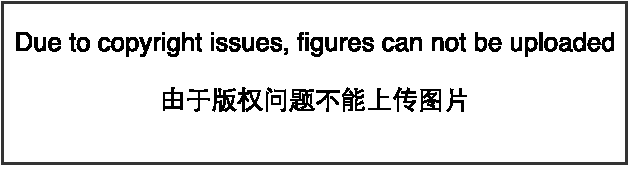
\includegraphics{figure.pdf}}
\else
\centerline{\includegraphics{Chapter15/figures/isomap_color}}
\fi
\caption{在\emph{函数空间}(并非参数空间,避免从参数向量到函数的多对一映射)不同神经网络的学习轨迹的非线性映射的可视化。
不同网络采用不同的随机初始化,并且有的使用了\gls{unsupervised_pretraining},有的没有。
每个点对应着训练过程中一个特定时间的神经网络。
经\citet{Erhan+al-2010-small}许可改编此图。
函数空间中的坐标是关于每组输入$\Vx$和它的一个输出$\Vy$的\gls{infinite}维向量。
\cite{Erhan+al-2010-small}将很多特定$\Vx$的$\Vy$连接起来,线性投影到高维空间中。
然后他们使用\gls{isomap}~\citep{Tenenbaum2000-isomap}进行进一步的非线性投影并投到二维空间。
颜色表示时间。
所有的网络初始化在上图的中心点附近(对应的函数区域在不多数输入上具有近似\gls{uniform_distribution}的类别$y$)。
随着时间推移,学习将函数向外移动到预测得更好的点。
当使用\gls{pretraining}时,训练会一致地收敛到同一个区域;
而不使用\gls{pretraining}时,训练会收敛到另一个不重叠的区域。
\gls{isomap}试图维持全局相对距离(体积因此也保持不变),因此使用\gls{pretraining}的模型对应的较小区域意味着,基于\gls{pretraining}的\gls{estimator}具有较小的方差。
}
\label{fig:chap15_isomap}
\end{figure}

% 525 head

% 525 end 

具有两个单独的训练阶段的另一个缺点是每个阶段都具有各自的\gls{hyperparameter}。
第二阶段的性能通常不能在第一阶段期间预测,因此在第一阶段提出\gls{hyperparameter}和第二阶段根据反馈来更新之间存在较长的延迟。
最通用的方法是在\gls{supervised}阶段使用\gls{validation_set}上的误差来挑选\gls{pretraining}阶段的\gls{hyperparameter},如\cite{Larochelle-jmlr-2009}中讨论的。
在实际中,有些\gls{hyperparameter},如\gls{pretraining}迭代的次数,很方便在\gls{pretraining}阶段设定,通过\gls{unsupervised}目标上使用\gls{early_stopping}策略完成。
这个策略并不理想,但是在计算上比使用\gls{supervised}目标代价小得多。

% 526 head

如今,大部分算法已经不使用\gls{unsupervised_pretraining}了,除了在\gls{NLP}领域中单词作为\gls{one_hot}向量的自然表示不能传达相似性信息,并且有非常多的\gls{unlabeled}数据集可用。
在这种情况下,\gls{pretraining}的优点是可以对一个巨大的\gls{unlabeled}集合(例如用包含数十亿单词的语料库)进行\gls{pretraining},学习良好的表示(通常是单词,但也可以是句子),然后使用该表示或\gls{fine_tune}它,使其适合于训练集样本大幅减少的\gls{supervised}任务。
这种方法由\cite{CollobertR2008-small}、\cite{Turian+Ratinov+Bengio-2010-small}和\cite{collobert2011natural}开创,至今仍在使用。

% 526 mid


基于\gls{supervised_learning}的\gls{DL}技术,通过\gls{dropout}或\gls{batch_normalization}来\gls{regularize},能够在很多任务上达到人类级别的性能,但仅仅是在极大的\gls{labeled}数据集上。
在中等大小的数据集(例如\ENNAME{CIFAR}-10和\ENNAME{MNIST},每个类大约有5,000个\gls{labeled}样本)上,这些技术的效果比\gls{unsupervised_pretraining}更好。
在极小的数据集,例如\gls{alternative_splicing_dataset},贝叶斯方法要优于基于\gls{unsupervised_pretraining}的方法~\citep{Srivastava-master-small}。
由于这些原因,\gls{unsupervised_pretraining}已经不如以前流行。
然而,\gls{unsupervised_pretraining}仍然是\gls{DL}研究历史上的一个重要里程碑,并将继续影响当代方法。
\gls{pretraining}的想法已经推广到\firstgls{supervised_pretraining},这将在\secref{sec:supervised_pretraining}中讨论,在\gls{transfer_learning}中这是非常常用的方法。
\gls{transfer_learning}中的\gls{supervised_pretraining}流行~\citep{Oquab-et-al-CVPR2014,yosinski-nips2014}于在\ENNAME{ImageNet}数据集上使用\gls{convolutional_network}\gls{pretraining}。
由于这个原因,实践者们公布了这些网络训练出的参数,就像自然语言任务公布\gls{pretraining}的单词向量一样~\citep{collobert2011natural,Mikolov-et-al-ICLR2013}。

% 526 end

\section{\glsentrytext{transfer_learning}和\glsentrytext{domain_adaption}}
\label{sec:transfer_learning_and_domain_adaptation}
\gls{transfer_learning}和\gls{domain_adaption}指的是利用一个情景(例如,分布$P_1$)中已经学到的内容去改善另一个情景(比如分布$P_2$)中的\gls{generalization}情况。
这点概括了上一节提出的想法,即在\gls{unsupervised_learning}任务和\gls{supervised_learning}任务之间转移表示。

%527 head

在\firstgls{transfer_learning}中,\gls{learner}必须执行两个或更多个不同的任务,但是我们假设能够解释$P_1$变化的许多因素和学习$P_2$需要抓住的变化相关。
这通常能够在\gls{supervised_learning}中解释,输入是相同的,但是输出不同的性质。
例如,我们可能在第一种情景中学习了一组视觉类别,比如猫和狗,然后在第二种情景中学习一组不同的视觉类别,比如蚂蚁和黄蜂。
如果第一种情景(从$P_1$采样)中具有非常多的数据,那么这有助于学习到能够使得从$P_2$抽取的非常少样本中快速\gls{generalize}的表示。%??
许多视觉类别\emph{共享}一些低级概念,比如边缘、视觉形状、几何变化、光照变化的影响等等。
一般而言,当存在对不同情景或任务有用特征时,并且这些特征对应多个情景出现的潜在因素,\gls{transfer_learning}、\gls{multitask_learning}(\secref{sec:multitask_learning})和\gls{domain_adaption}可以使用\gls{representation_learning}来实现。
如\figref{fig:chap7_multi_factor_output}所示,这是具有共享底层和任务相关上层的学习框架。

% 527 mid

然而,有时不同任务之间共享的不是输入的语义,而是输出的语义。
例如,\gls{SR}系统需要在输出层产生有效的句子,但是输入附近的较低层可能需要识别相同\gls{phoneme}或子\gls{phoneme}发音的非常不同的版本(这取决于说话人)。
在这样的情况下,共享神经网络的上层(输出附近)和进行任务特定的预处理是有意义的,如\figref{fig:chap15_multi_task_input}所示。

% 527 mid

% 528 head

\begin{figure}[!htb]
\ifOpenSource
\centerline{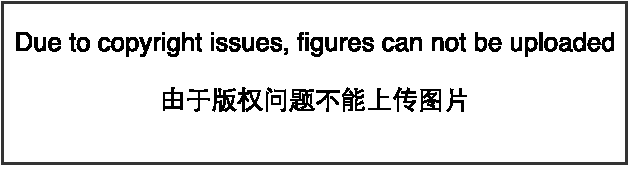
\includegraphics{figure.pdf}}
\else
\centerline{\includegraphics{Chapter15/figures/multi_task_input}}
\fi
\caption{\gls{multitask_learning}或者\gls{transfer_learning}的架构示例。
输出变量$\RVy$在所有的任务上具有相同的语义;输入变量$\RVx$在每个任务(或者,比如每个用户)上具有不同的意义(甚至可能具有不同的维度),图上三个任务为$\RVx^{(1)}$,$\RVx^{(2)}$,$\RVx^{(3)}$。
底层结构(决定了选择方向)是面向任务的,上层结构是共享的。
底层结构学习将面向特定任务的输入转化为通用特征。
}
\label{fig:chap15_multi_task_input}
\end{figure}

% 528 head

在\firstgls{domain_adaption}的相关情况下,在每个情景之间任务(和最优的输入到输出的映射)都是相同的,但是\gls{input_distribution}稍有不同。 
例如,考虑情感分析的任务,如判断一条评论是表达积极的还是消极的情绪。 
网上的评论有许多类别。
在书、视频和音乐等媒体内容上训练的顾客评论情感预测器,被用于分析诸如电视机或智能电话的消费电子产品的评论时,\gls{domain_adaption}情景可能会出现。%?? 
可以想象,存在一个潜在的函数可以判断任何语句是正面的、中性的还是负面的,但是词汇和风格可能会因领域而有差异,使得跨域的\gls{generalize}训练变得更加困难。
简单的\gls{unsupervised_pretraining}(\gls{DAE})已经能够非常成功地用于\gls{domain_adaption}的情感分析\citep{Glorot+al-ICML-2011}。
% 527 end 

% 528 head

一个相关的问题是\firstgls{concept_drift},我们可以将其视为一种\gls{transfer_learning},因为数据分布随时间而逐渐变化。
\gls{concept_drift}和\gls{transfer_learning}都可以被视为\gls{multitask_learning}的特定形式。
``\gls{multitask_learning}''这个术语通常指\gls{supervised_learning}任务,而更广义的\gls{transfer_learning}的概念也适用于\gls{unsupervised_learning}和\gls{RL}。

% 528 mid

在所有这些情况下,我们的目标是利用第一个\gls{setting}下的数据,提取那些在第二种\gls{setting}中学习时或直接进行预测时可能有用的信息。
\gls{representation_learning}的核心思想是相同的表示可能在两种\gls{setting}中都是有用的。
两个\gls{setting}使用相同的表示,使得表示可以受益于两个任务的训练数据。

% 528 end

如前所述,\gls{transfer_learning}中\gls{unsupervised}\gls{DL}已经在一些\gls{ML}比赛中取得了成功~\citep{UTLC+LISA-2011-small,goodfellow+all-NIPS2011}。
这些比赛中的某一个实验配置如下。
首先每个参与者获得一个第一种\gls{setting}(来自分布$P_1$)的数据集,其中含有一些类别的样本。
参与者必须使用这个来学习一个良好的特征空间(将原始输入映射到某种表示),使得当我们将这个\gls{learned}变换用于来自迁移\gls{setting}(分布$P_2$)的输入时,\gls{linear_classifier}可以在很少\gls{labeled}样本上训练、并\gls{generalize}得很好。
这个比赛中最引人注目的结果之一是,学习表示的网络架构越深(在第一个\gls{setting}$P_1$中的数据使用纯\gls{unsupervised}方式学习),在第二个\gls{setting}(迁移)$P_2$的新类别上学习到的曲线就越好。
对于深度表示而言,迁移任务只需要少量\gls{labeled}样本就能显著地提升\gls{generalization}性能。

% 529 head

\gls{transfer_learning}的两种极端形式是\firstgls{one_shot_learning}和\firstgls{zero_shot_learning},有时也被称为\firstgls{zero_data_learning}。
只有一个\gls{labeled}样本的迁移任务被称为\gls{one_shot_learning};没有\gls{labeled}样本的迁移任务被称为\gls{zero_shot_learning}。

% 529 mid

因为第一阶段学习出的表示就可以清楚地分离出潜在的类别,所以\gls{one_shot_learning}~\citep{Fei-Fei+al-2006}是可能的。
在\gls{transfer_learning}阶段,仅需要一个\gls{labeled}样本来推断表示空间中聚集在相同点周围许多可能测试样本的\gls{label}。
这使得在\gls{learned}的表示空间中,对应于不变性的变化因子已经与其他因子完全分离,在区分某些类别的对象时,我们可以学习到哪些因素具有决定意义。

% 529 mid

考虑一个\gls{zero_shot_learning}\gls{setting}的例子,\gls{learner}已经读取了大量文本,然后要解决\gls{object_recognition}的问题。
如果文本足够好地描述了对象,那么即使没有看到某对象的图像,也能识别出该对象的类别。
例如,已知猫有四条腿和尖尖的耳朵,那么\gls{learner}可以在没有见过猫的情况下猜测该图像中是猫。

% 529 end


只有在训练时使用了额外信息,\gls{zero_data_learning}~\citep{Larochelle2008}和\gls{zero_shot_learning}~\citep{Palatucci2009,Socher-2013}才是有可能的。
我们可以认为\gls{zero_data_learning}场景包含三个随机变量:传统输入$\Vx$,传统输出或目标$\Vy$,以及描述任务的附加随机变量$T$。
该模型被训练来估计条件分布$p(\Vy \mid \Vx, T)$,其中$T$是我们希望执行的任务的描述。
在我们的例子中,读取猫的文本信息然后识别猫,输出是二元变量$y$,$y=1$表示``是'',$y=0$表示``不是''。
任务变量$T$表示要回答的问题,例如``这个图像中是否有猫?''
如果训练集包含和$T$在相同空间的\gls{unsupervised}对象样本,我们也许能够推断未知的$T$实例的含义。
在我们的例子中,没有提前看到猫的图像而去识别猫,所以拥有一些\gls{unlabeled}文本数据包含句子诸如``猫有四条腿''或``猫有尖耳朵'',对于学习非常有帮助。

% 530  head

\gls{zero_shot_learning}要求$T$被表示为某种形式的\gls{generalization}。
例如,$T$不能仅是指示对象类别的\gls{one_hot}编码。
通过使用每个类别词的\gls{word_embeddings}表示,\cite{Socher-2013}提出了对象类别的\gls{distributed_representation}。

% 530 mid

我们还可以在\gls{machine_translation}中发现一种类似的现象~\citep{Klementiev-et-al-COLING2012,Mikolov-et-al-arxiv2013,Gouws-et-al-arxiv2014}:我们已经知道一种语言中的单词,还可以学到单一语言语料库中词与词之间的关系;另一方面,我们已经翻译了一种语言中的单词与另一种语言中的单词相关的句子。
即使我们可能没有将语言$X$中的单词$A$翻译成语言$Y$中的单词$B$的\gls{labeled}样本,我们也可以\gls{generalize}并猜出单词$A$的翻译,这是由于我们已经学习了语言$X$和$Y$单词的\gls{distributed_representation},并且通过两种语言句子的匹配对组成的训练样本,产生了关联于两个空间的链接(可能是双向的)。
如果联合学习三种成分(两种表示形式和它们之间的关系),那么这种迁移将会非常成功。

% 530 mid

\gls{zero_shot_learning}是\gls{transfer_learning}的一种特殊形式。
同样的原理可以解释如何能执行\firstgls{multimodal_learning},学习两种\gls{modality}的表示,和一种\gls{modality}中的观察结果$\Vx$与另一种\gls{modality}中的观察结果$\Vy$组成的对$(\Vx, \Vy)$之间的关系(通常是一个联合分布)\citep{Srivastava+Salakhutdinov-NIPS2012-small}。
通过学习所有的三组参数(从$\Vx$到它的表示、从$\Vy$到它的表示,以及两个表示之间的关系),一个表示中的概念被锚定在另一个表示中,反之亦然,从而可以有效地推广到新的对组。 %?? allowing one 
这个过程如\figref{fig:chap15_maps_between_representations}所示。

% 530 end

% 531

\begin{figure}[!htb]
\ifOpenSource
\centerline{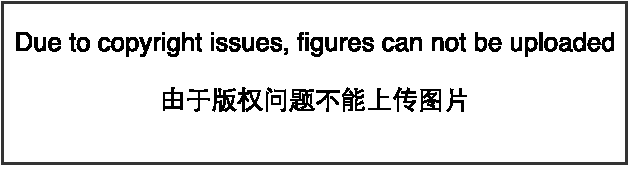
\includegraphics{figure.pdf}}
\else
\centerline{\includegraphics{Chapter15/figures/maps_between_representations}}
\fi
\caption{两个域$\Vx$和$\Vy$之间的\gls{transfer_learning}能够进行\gls{zero_shot_learning}。
\gls{labeled}或\gls{unlabeled}样本$\Vx$可以学习表示函数$f_{\Vx}$。
同样地,样本$\Vy$也可以学习表示函数$f_{\Vy}$。
上图中$f_{\Vx}$和$f_{\Vy}$旁都有一个向上的箭头,不同的箭头表示不同的作用函数。
并且箭头的类型表示使用了哪一种函数。
$\Vh_{\Vx}$空间中的相似性度量表示$\Vx$空间中任意点对之间的距离,这种度量方式比直接度量$\Vx$空间的距离更好。
同样地,$\Vh_{\Vy}$空间中的相似性度量表示$\Vy$空间中任意点对之间的距离。
这两种相似函数都使用带点的双向箭头表示。
\gls{labeled}样本(水平虚线)$(\Vx, \Vy)$能够学习表示$f_{\Vx}(\Vx)$和表示$f_{\Vy}(\Vy)$之间的单向或双向映射(实双向箭头),以及这些表示之间如何锚定。
\gls{zero_data_learning}可以通过以下方法实现。
像$\Vx_{\text{test}}$可以和单词$\Vy_{\text{test}}$关联起来,即使该单词没有像,仅仅是因为单词表示$f_{\Vy}(\Vy_{\text{test}})$和像表示$f_{\Vx}(\Vx_{\text{test}})$可以通过表示空间的映射彼此关联。
这种方法有效的原因是,尽管像和单词没有匹配成队,但是它们各自的特征向量$f_{\Vx}(\Vx_{\text{test}})$和$f_{\Vy}(\Vy_{\text{test}})$互相关联。
上图受\ENNAME{Hrant Khachatrian}的建议启发。
}
\label{fig:chap15_maps_between_representations}
\end{figure}

% 531

\section{\glsentrytext{semi_supervised}解释因果关系}
\label{sec:semi_supervised_disentangling_of_causal_factors}

% 532 head

\gls{representation_learning}的一个重要问题是``什么原因能够使一个表示比另一个表示更好?''
一种假设是,理想表示中的特征对应到观测数据的\gls{underlying_cause},特征空间中不同的特征或方向对应着不同的原因,从而表示能够区分这些原因。
这个假设促使我们去寻找表示$p(\Vx)$的更好方法。
如果$\Vy$是$\Vx$的重要成因之一,那么这种表示也可能是计算$p(\Vy \mid \Vx)$的一种良好表示。
从20世纪90年代以来,这个想法已经指导了大量的\gls{DL}研究工作~\citep{Becker92,hinton1999unsupervised}。
关于\gls{semi_supervised_learning}可以超过纯\gls{supervised_learning}的其他论点,请读者参考\cite{Chapelle-2006}的第1.2节。

% 532 head

在\gls{representation_learning}的其他方法中,我们大多关注易于建模的表示——例如,数据稀疏或是各项之间相互独立的情况。
能够清楚地分离出潜在因素的表示可能并不一定易于建模。
然而,该假设促使\gls{semi_supervised_learning}使用\gls{unsupervised}\gls{representation_learning}的一个更深层原因是,对于很多\gls{AI}任务而言,有两个相随的特点:一旦我们能够获得观察结果基本成因的解释,那么将会很容易分离出个体属性。
具体来说,如果表示向量$\Vh$表示观察值$\Vx$的很多潜在因素,并且输出向量$\Vy$是最为重要的原因之一,那么从$\Vh$预测$\Vy$会很容易。

% 532 mid 

首先,让我们看看$p(\RVx)$的\gls{unsupervised_learning}无助于学习$p(\RVy\mid\RVx)$时,\gls{semi_supervised_learning}为何失败。
例如,考虑一种情况,$p(\RVx)$是均匀分布的,我们希望学习$f(\Vx) = \SetE[\RVy \mid \Vx]$。
显然,仅仅观察\gls{training_set}的值$\Vx$不能给我们关于$p(\RVy \mid \RVx)$的任何信息。

% 532 mid 

接下来,让我们看看\gls{semi_supervised_learning}成功的一个简单例子。
考虑这样的情况,$\RVx$来自一个混合分布,每个$\RVy$值具有一个混合分量,如\figref{fig:chap15_mixture_model}所示。
如果混合分量很好地分出来了,那么建模$p(\RVx)$可以精确地指出每个分量的位置,每个类一个\gls{labeled}样本的\gls{training_set}足以精确学习$p(\RVy \mid \RVx)$。
但是更一般地,什么能将$p(\RVy \mid \RVx)$和$p(\RVx)$关联在一起呢?

% 532 mid-end

% 533 head

\begin{figure}[!htb]
\ifOpenSource
\centerline{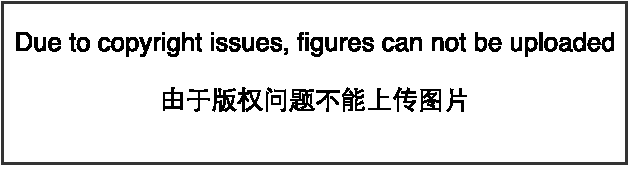
\includegraphics{figure.pdf}}
\else
\centerline{\includegraphics{Chapter15/figures/mixture_model_color}}
\fi
\caption{混合模型。具有三个混合分量的$x$上混合密度示例。
混合分量的内在本质是潜在\gls{explanatory_factor}$y$。
因为混合分量(例如,图像数据中的自然对象类别)在统计学上是显著的,所以仅仅使用\gls{unlabeled}样本\gls{unsupervised}建模$p(x)$也能揭示\gls{explanatory_factor}$y$。
}
\label{fig:chap15_mixture_model}
\end{figure}

% 533 head


如果$\RVy$与$\RVx$的成因之一非常相关,那么$p(\RVx)$和$p(\RVy \mid \RVx)$也会紧密关联,试图找到变化\gls{underlying}因素的\gls{unsupervised}\gls{representation_learning}可能像\gls{semi_supervised_learning}一样有用。

% -- 532 end

% 533 mid

假设$\RVy$是$\RVx$的成因之一,让$\RVh$代表所有这些成因。
真实的生成过程可以被认为是根据这个\gls{directed_graphical_model}结构化出来的,其中$\RVh$是$\RVx$的父节点:
\begin{equation}
	p(\RVh, \RVx) = p(\RVx \mid \RVh) p(\RVh).
\end{equation} % 533 mid
因此,数据的边缘概率是
\begin{equation}
	p(\Vx) = \SetE_{\RVh} p(\Vx \mid \Vh).
\end{equation}
从这个直观的观察中,我们得出结论,$\RVx$最好可能的模型(从广义的观点)是会表示上述``真实''结构的,其中$\Vh$作为\gls{latent_variable}解释$\Vx$中可观察的变化。
上文讨论的``理想''的\gls{representation_learning}应该能够反映出这些\gls{latent}因子。
如果$\RVy$是其中之一(或是紧密关联于其中之一),那么将很容易从这种表示中预测$\RVy$。
我们会看到给定$\RVx$下$\RVy$的条件分布通过\gls{bayes_rule}关联到上式中的分量:
\begin{equation}
	p(\RVy \mid \RVx) = \frac{ p(\RVx \mid \RVy) p(\RVy) }{p(\RVx)}.
\end{equation}
因此边缘概率$p(\RVx)$和条件概率$p(\RVy \mid \RVx)$密切相关,前者的结构信息应该有助于学习后者。
因此,在这些假设情况下,\gls{semi_supervised_learning}应该能提高性能。

% 533 end

关于这个事实的一个重要的研究问题是,大多数观察是由极其大量的\gls{underlying_cause}形成的。
假设$\RVy = \RSh_i$,但是\gls{unsupervised}\gls{learner}并不知道是哪一个$\RSh_i$。
对于一个\gls{unsupervised}\gls{learner}暴力求解就是学习一种表示,这种表示能够捕获\emph{所有}合理的重要生成因子$\RSh_j$,并将它们彼此区分开来,因此不管$\RSh_i$是否关联于$\RVy$,从$\RVh$预测$\RVy$都是容易的。

% -- 534 head

在实践中,暴力求解是不可行的,因为不可能捕获影响观察的所有或大多数变化因素。
例如,在视觉场景中,表示是否应该对背景中的所有最小对象进行编码?
根据一个有据可查的心理学现象,人们不会察觉到环境中和他们所在进行的任务并不立刻相关的变化,具体例子可以参考\cite{simons1998failure}。
\gls{semi_supervised_learning}的一个重要研究前沿是确定每种情况下要编码\emph{什么}。
目前,处理大量\gls{underlying}原因的两个主要策略是,同时使用\gls{unsupervised_learning}和\gls{supervised_learning}信号,从而使得模型捕获最相关的变动因素,或是使用纯\gls{unsupervised_learning}学习更大规模的表示。

% 534 mid

\gls{unsupervised_learning}的另一个思路是选择一个更好的确定哪些\gls{underlying}因素最为关键的定义。
之前,\gls{AE}和\gls{generative_model}被训练来优化一个类似于\gls{mean_squared_error}的固定标准。
这些固定标准确定了哪些因素是重要的。
例如,图像像素的\gls{mean_squared_error}隐式地指定,一个\gls{underlying}因素只有在其显著地改变大量像素的亮度时,才是重要影响因素。
如果我们希望解决的问题涉及到小对象之间的相互作用,那么这将有可能遇到问题。
如\figref{fig:chap15_pingpong}所示,在机器人任务中,\gls{AE}未能学习到编码小乒乓球。
同样是这个机器人,它可以成功地与更大的对象进行交互(例如棒球,\gls{mean_squared_error}在这种情况下很显著)。

% 534 mid

% 535 head

\begin{figure}[!htb]
\ifOpenSource
\centerline{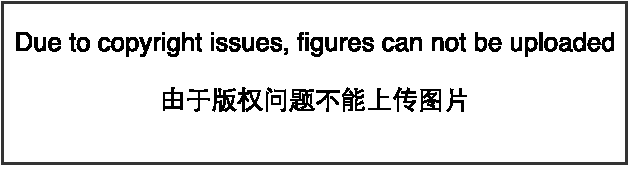
\includegraphics{figure.pdf}}
\else
\begin{tabular}{cc}
输入 & 重构 \\
\includegraphics[width=0.45\textwidth]{Chapter15/figures/ping_pong_input} &
\includegraphics[width=0.45\textwidth]{Chapter15/figures/ping_pong_reconstruction}
\end{tabular}
\fi
\caption{机器人任务上,基于\gls{mean_squared_error}训练的\gls{AE}不能重构乒乓球。
乒乓球的存在及其所有空间坐标,是生成图像且与机器人任务相关的重要潜在因素。
不幸的是,\gls{AE}具有有限的容量,基于\gls{mean_squared_error}的训练没能将乒乓球作为显著物体识别出来编码。
以上图像由Chelsea Finn提供。
}
\label{fig:chap15_pingpong}
\end{figure}

% 535 head

% 534 end

还有一些其他的显著性的定义。
例如,如果一组像素具有高度可识别的模式,那么即使该模式不涉及到极端的亮度或暗度,该模式还是会被认为非常显著。
实现这样一种定义显著的方法是使用最近提出的\firstgls{generative_adversarial_networks}~\citep{Goodfellow-et-al-NIPS2014-small}。
在这种方法中,\gls{generative_model}被训练来愚弄\gls{feedforward_classifier}。
\gls{feedforward_classifier}尝试将来自\gls{generative_model}的所有样本识别为假的,并将来自\gls{training_set}的所有样本识别为真的。
在这个框架中,\gls{feedforward_network}能够识别出的任何结构化模式都是非常显著的。
\gls{generative_adversarial_networks}会在\secref{sec:generative_adversarial_networks}中更详细地介绍。
为了叙述方便,知道它能\emph{学习}出如何决定什么是显著的就可以了。
\cite{lotter2015unsupervised}表明,生成人类头部头像的模型在使用\gls{mean_squared_error}训练时往往会忽视耳朵,但是\gls{adversarial}式框架学习能够成功地生成耳朵。
因为耳朵与周围的皮肤相比不是非常明亮或黑暗,所以根据\gls{mean_squared_error}损失它们不是特别突出,但是它们高度可识别的形状和一致的位置意味着\gls{feedforward_network}能够轻易地学习出如何检测它们,从而使得它们在\gls{generative_adversarial_framework}下是高度突出的。
\figref{fig:chap15_manface}给了一些样例图片。
\gls{generative_adversarial_networks}只是确定应该表示哪些因素的一小步。
我们期望未来的研究能够发现更好的方式来确定表示哪些因素,并且根据任务来开发表示不同因素的机制。

% -- 535 mid


% 536 head
\begin{figure}[!htb]
\ifOpenSource
\centerline{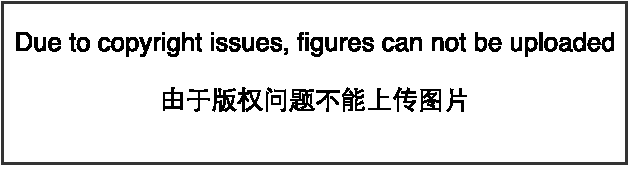
\includegraphics{figure.pdf}}
\else
\begin{tabular}{ccc}
真实图 & \glssymbol{mean_squared_error} & 对抗学习 \\
\includegraphics[width=0.3\textwidth]{Chapter15/figures/PGN_face1_GT} &
\includegraphics[width=0.3\textwidth]{Chapter15/figures/PGN_face1_MSE} &
\includegraphics[width=0.3\textwidth]{Chapter15/figures/PGN_face1_AL}
\end{tabular}
\fi
\caption{
预测生成网络是一个学习哪些特征显著的例子。
在这个例子中,预测生成网络已被训练成在特定视角预测人头的3D模型。
\emph{(左)}真实情况。
这是一张网络应该生成的正确图片。
\emph{(中)}由具有\gls{mean_squared_error}的预测生成网络生成的图片。
因为与相邻皮肤相比,耳朵不会引起亮度的极大差异,所以它们的显著性不足以让模型学习表示它们。
\emph{(右)}由具有\gls{mean_squared_error}和对抗损失的模型生成的图片。
使用这个\gls{learned}的\gls{cost_function},由于耳朵遵循可预测的模式,因此耳朵是显著重要的。
学习哪些原因对于模型而言是足够重要和相关的,是一个重要的活跃研究领域。
以上图片由\cite{lotter2015unsupervised}提供。
}
\label{fig:chap15_manface}
\end{figure}
% 536 head


% 535 head

正如\cite{Janzing-et-al-ICML2012}指出,学习\gls{underlying}因素的好处是,如果真实的生成过程中$\RVx$是结果,$\RVy$是原因,那么建模$p(\RVx \mid \RVy)$对于$p(\RVy)$的变化是鲁棒的。
如果因果关系被逆转,这是不对的,因为根据\gls{bayes_rule},$p(\RVx \mid \RVy)$将会对$p(\RVy)$的变化十分敏感。
很多时候,我们考虑分布的变化(由于不同领域、时间不稳定性或任务性质的变化)时,\emph{因果机制是保持不变的}(``宇宙定律不变''),而\gls{underlying}因素的边缘分布是会变化的。
因此,通过学习试图恢复成因向量$\RVh$和$p(\RVx \mid \RVh)$的\gls{generative_model},我们可以期望最后的模型对所有种类的变化有更好的\gls{generalization}和鲁棒性。

% 536 mid

\section{\glsentrytext{distributed_representation}}
\label{sec:distributed_representation}
% 536 end

\gls{distributed_representation}的概念(由很多元素组合的表示,这些元素之间可以设置成可分离的)是\gls{representation_learning}最重要的工具之一。
\gls{distributed_representation}非常强大,因为他们能用具有$k$个值的$n$个特征去描述$k^n$个不同的概念。
正如我们在本书中看到的,具有多个\gls{hidden_unit}的\gls{NN}和具有多个\gls{latent_variable}的概率模型都利用了\gls{distributed_representation}的策略。
我们现在再介绍一个观察结果。
许多\gls{DL}算法基于的假设是,\gls{hidden_unit}能够学习表示出解释数据的\gls{underlying}\gls{causal_factor},就像\secref{sec:semi_supervised_disentangling_of_causal_factors}中讨论的一样。
这种方法在\gls{distributed_representation}上是自然的,因为表示空间中的每个方向都对应着一个不同的\gls{underlying}配置变量的值。

%  537 head

$n$维二元向量是一个\gls{distributed_representation}的示例,有$2^n$种配置,每一种都对应输入空间中的一个不同区域,如\figref{fig:chap15_distributed}所示。
这可以与\emph{\gls{symbolic_representation}}相比较,其中输入关联到单一符号或类别。
如果字典中有$n$个符号,那么可以想象有$n$个特征监测器,每个特征探测器监测相关类别的存在。
在这种情况下,只有表示空间中$n$个不同配置才有可能在输入空间中刻画$n$个不同的区域,如\figref{fig:chap15_nondistributed}所示。
这样的\gls{symbolic_representation}也被称为\gls{one_hot}表示,因为它可以表示成相互排斥的$n$维二元向量(其中只有一位是激活的)。
\gls{symbolic_representation}是更广泛的\gls{nondistributed_representation}类中的一个具体示例,它可以包含很多条目,但是每个条目没有显著意义的单独控制作用。

% 537 mid

% 538 1 page

\begin{figure}[!htb]
\ifOpenSource
\centerline{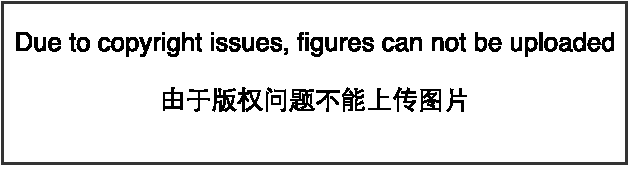
\includegraphics{figure.pdf}}
\else
\centerline{\includegraphics{Chapter15/figures/distributed}}
\fi
\caption{基于\gls{distributed_representation}的学习算法如何将输入空间分割成多个区域的图示。
这个例子具有二元变量$h_1$,$h_2$,$h_3$。
每个特征通过为\gls{learned}的线性变换设定输出阀值而定义。
每个特征将$\SetR^2$分成两个半平面。
令$h_i^+$表示输入点$h_i=1$的集合;$h_i^-$表示输入点$h_i=0$的集合。
在这个图示中,每条线代表着一个$h_i$的决策边界,对应的箭头指向边界的$h_i^+$区域。
整个表示在这些半平面的每个相交区域都指定一个唯一值。
例如,表示值为$[1,1,1]^\top$对应着区域$h_1^+ \cap h_2^+ \cap h_3^+$。
可以将以上表示和\figref{fig:chap15_nondistributed}中的\gls{nondistributed_representation}进行比较。
在输入维度是$d$的一般情况下,\gls{distributed_representation}通过半空间(而不是半平面)的交叉分割$\SetR^d$。
具有$n$个特征的\gls{distributed_representation}给$O(n^d)$个不同区域分配唯一的编码,而具有$n$个样本的\gls{nearest_neighbor}算法只能给$n$个不同区域分配唯一的编码。
因此,\gls{distributed_representation}能够比\gls{nondistributed_representation}多分配指数级的区域。
注意并非所有的$\Vh$值都是可取的(这个例子中没有$\Vh=\mathbf{0}$),在\gls{distributed_representation}上的\gls{linear_classifier}不能向每个相邻区域分配不同的类别标识;
甚至深度线性阀值网络的\glssymbol{VC}维只有$O(w\log w)$(其中$w$是权重数目)\citep{sontag1998vc}。
强表示层和弱分类器层的组合是一个强\gls{regularizer}。
试图学习``人''和``非人''概念的分类器不需要给表示为``戴眼镜的女人''和``没有戴眼镜的男人''的输入分配不同的类别。
容量限制鼓励每个分类器关注少数几个$h_i$,鼓励$\Vh$以线性可分的方式学习表示这些类别。
}
\label{fig:chap15_distributed}
\end{figure}

% 538 1 page

% 539 head

\begin{figure}[!htb]
\ifOpenSource
\centerline{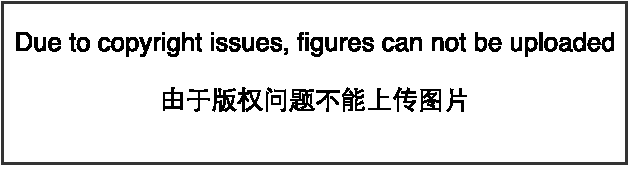
\includegraphics{figure.pdf}}
\else
\centerline{\includegraphics{Chapter15/figures/non_distributed}}
\fi
\caption{\gls{nearest_neighbor}算法如何将输入空间分成不同区域的图示。
\gls{nearest_neighbor}算法是一个基于\gls{nondistributed_representation}的学习算法的示例。
不同的\gls{nondistributed}算法可以具有不同的几何形状,但是它们通常将输入空间分成区域,\emph{每个区域具有不同的参数}。
\gls{nondistributed}方法的优点是,给定足够的参数,它能够拟合一个\gls{training_set},而不需要复杂的优化算法。
因为它直接为每个区域\emph{独立地}设置不同的参数。
缺点是,\gls{nondistributed_representation}的模型只能通过平滑先验来局部地\gls{generalize},因此学习波峰波谷多于样本的复杂函数时,该方法是不可行的。
和\gls{distributed_representation}的对比,可以参照\figref{fig:chap15_distributed}。
}
\label{fig:chap15_nondistributed}
\end{figure}

% 539 head


% 537 mid

以下是基于\gls{nondistributed_representation}的学习算法的示例:
\begin{itemize}
	\item 聚类算法,包含$k$-means算法:每个输入点恰好分配到一个类别。

	\item $k$-\gls{nearest_neighbor}算法:给定一个输入,一个或几个模板或原型样本与之关联。
	在$k >  1$ 的情况下,每个输入都使用多个值来描述,但是它们不能彼此分开控制,因此这不能算真正的\gls{distributed_representation}。

	\item \gls{decision_tree}:给定输入时,只有一个叶节点(和从根到该叶节点路径上的点)是被激活的。

	\item \gls{gauss_mixture}和\gls{mixture_of_experts}:模板(聚类中心)或专家关联一个激活的\emph{程度}。
	和$k$-\gls{nearest_neighbor}算法一样,每个输入用多个值表示,但是这些值不能轻易地彼此分开控制。

	\item 具有\gls{gaussian_kernel} (或其他类似的\gls{local_kernel})的\gls{kernel_machines}: 尽管每个``\gls{support_vectors}''或模板样本的激活程度是连续值,但仍然会出现和\gls{gauss_mixture}相同的问题。

% 537 end

	\item 基于\gls{n_gram}的语言或翻译模型:根据后缀的树结构划分上下文集合(符号序列)。
	例如,一个叶节点可能对应于最后两个单词$w_1$和$w_2$。
	树上的每个叶节点分别估计单独的参数(有些共享也是可能的)。
\end{itemize}

% -- 539 mid  



对于部分\gls{nondistributed}算法而言,有些输出并非是恒定的,而是在相邻区域之间内插。
参数(或样本)的数量和它们能够定义区域的数量之间仍保持线性关系。

% -- 539 mid  

将\gls{distributed_representation}和\gls{symbolic_representation}区分开来的一个重要概念是,由不同概念之间的\emph{共享属性而产生的\gls{generalization}}。
作为纯符号,``猫''和``狗''之间的距离和任意其他两种符号的距离一样。
然而,如果将它们与有意义的\gls{distributed_representation}相关联,那么关于猫的很多特点可以推广到狗,反之亦然。
例如,我们的\gls{distributed_representation}可能会包含诸如``具有皮毛''或``腿的数目''这类在``猫''和``狗''的嵌入上具有相同值的项。
正如\secref{sec:neural_language_models}所讨论的,作用于单词\gls{distributed_representation}的神经语言模型比其他直接对单词\gls{one_hot}表示进行操作的模型\gls{generalize}得更好。
\gls{distributed_representation}具有丰富的\emph{相似性空间},语义上相近的概念(或输入)在距离上接近,这是纯粹的\gls{symbolic_representation}所缺少的特点。

% -- 540 head

在学习算法中使用\gls{distributed_representation}何时以及为什么具有统计优势?
当一个明显复杂的结构可以用较少参数紧致地表示时,\gls{distributed_representation}具有统计上的优点。
一些传统的\gls{nondistributed}学习算法仅仅在平滑假设的情况下能够\gls{generalize},也就是说如果$u\approx v$,那么学习到的目标函数$f$通常具有$f(u) \approx f(v)$的性质。
有许多方法来形式化这样一个假设,但其结果是如果我们有一个样本$(x,y)$,并且我们知道$f(x) \approx y$,那么我们可以选取一个\gls{estimator}$\hat{f}$近似地满足这些限制,并且当我们移动到附近的输入$x + \epsilon$时,$\hat{f}$尽可能少地发生改变。
显然这个假设是非常有用的,但是它会遭受\gls{curse_of_dimensionality}:
学习出一个能够在很多不同区域上增加或减少很多次的目标函数
\footnote{一般来说,我们可能会想要学习一个函数,这个函数在指数级数量区域的表现都是不同的:在$d$-维空间中,为了区分每一维,至少有两个不同的值。
我们想要函数$f$区分这$2^d$个不同的区域,需要$O(2^d)$量级的训练样本},
我们可能需要至少和可区分区域数量一样多的样本。
我们可以将每一个区域视为一个类别或符号:通过让每个符号(或区域)具有单独的自由度,我们可以学习出从符号映射到值的任意\gls{decoder}。
然而,这不能推广到新区域的新符号上。

% -- 540 mid

如果我们幸运的话,除了平滑之外,目标函数可能还有一些其他规律。
例如,具有\gls{max_pooling}的\gls{convolutional_network}可以在不考虑对象在图像中位置(即使对象的空间变换不对应输入空间的平滑变换)的情况下识别出对象。

% -- 540 mid

让我们检查\gls{distributed_representation}学习算法的一个特殊情况,它通过对输入的线性函数进行阀值处理来提取二元特征。
该表示中的每个二元特征将$\SetR^d$分成一对半空间,如\figref{fig:chap15_distributed}所示。
$n$个相应半空间的指数级数量的交集确定了该\gls{distributed_representation}\gls{learner}能够区分多少区域。
空间$\SetR^d$中的$n$个超平面的排列组合能够生成多少区间?
通过应用关于超平面交集的一般结果~\citep{Zaslavsky-1975},我们发现~\citep{Pascanu+et+al-ICLR2014b}这个二元特征表示能够区分的空间数量是
\begin{equation}
	\sum_{j=0}^d \binom{n}{j} = O(n^d).
\end{equation}
因此,我们会发现关于输入大小呈指数级增长,关于\gls{hidden_unit}的数量呈多项式级增长。

% -- 541 head

这提供了\gls{distributed_representation}\gls{generalization}能力的一种几何解释:$O(nd)$个参数(空间$\SetR^d$中的$n$个线性阀值特征)能够明确表示输入空间中$O(n^d)$个不同区域。
如果我们没有对数据做任何假设,并且每个区域使用唯一的符号来表示,每个符号使用单独的参数去识别$\SetR^d$中的对应区域,那么指定$O(n^d)$个区域需要$O(n^d)$个样本。
更一般地,\gls{distributed_representation}的优势还可以体现在我们对\gls{distributed_representation}中的每个特征使用非线性的、可能连续的\gls{feature_extractor},而不是\gls{linear_threshold_units}的情况。
在这种情况下,如果具有$k$个参数的参数变换可以学习输入空间中的$r$个区域($k\ll r$),并且如果学习这样的表示有助于关注的任务,那么这种方式会比\gls{nondistributed}\gls{setting}(我们需要$O(r)$个样本来获得相同的特征,将输入空间相关联地划分成$r$个区域。)\gls{generalize}得更好。
使用较少的参数来表示模型意味着我们只需拟合较少的参数,因此只需要更少的训练样本去获得良好的\gls{generalization}。

% -- 541 mid

另一个解释基于\gls{distributed_representation}的模型\gls{generalization}能力更好的说法是,尽管能够明确地编码这么多不同的区域,但它们的\gls{capacity}仍然是很有限的。
例如,\gls{linear_threshold_units}\gls{NN}的\glssymbol{VC}维仅为$O(w\log w)$, 其中$w$是权重的数目~\citep{sontag1998vc}。
这种限制出现的原因是,虽然我们可以为表示空间分配非常多的唯一码,但是我们不能完全使用所有的码空间,也不能使用\gls{linear_classifier}学习出从表示空间$\Vh$到输出$\Vy$的任意函数映射。
因此使用与\gls{linear_classifier}相结合的\gls{distributed_representation}传达了一种先验信念,待识别的类在$\Vh$代表的\gls{underlying}\gls{causal_factor}的函数下是线性可分的。
我们通常想要学习类别,例如所有绿色对象的图像集合,或是所有汽车图像集合,但不会是需要非线性\ENNAME{XOR}逻辑的类别。
例如,我们通常不会将数据划分成所有红色汽车和绿色卡车作为一个集合,所有绿色汽车和红色卡车作为另一个集合。

% -- 542 head

到目前为止讨论的想法都是抽象的,但是它们可以通过实验验证。
\cite{Zhou-et-al-ICLR2015}发现,在\ENNAME{ImageNet}和\ENNAME{Places}基准数据集上训练的深度\gls{convolutional_network}中的\gls{hidden_unit}\gls{learned}的特征通常是可以解释的,对应人类自然分配的\gls{label}。
在实践中,\gls{hidden_unit}并不能总是学习出具有简单语言学名称的事物,但有趣的是,这些事物会在那些最好的\gls{CV}深度网络的顶层附近出现。
这些特征的共同之处在于,我们可以设想\emph{学习其中的每个特征不需要知道所有其他特征的所有配置}。
\cite{radford2015unsupervised}发现\gls{generative_model}可以学习人脸图像的表示,在表示空间中的不同方向捕获不同的\gls{underlying}\gls{factors_of_variation}。
\figref{fig:chap15_generative_glasses}展示表示空间中的一个方向对应着该人是男性还是女性,而另一个方向对应着该人是否戴着眼镜。
这些特征都是自动发现的,而非先验固定的。
我们没有必要为\gls{hidden_unit}分类器提供\gls{label}:只要该任务需要这样的特征,\gls{GD}就能在感兴趣的\gls{objective_function}上自然地学习出语义上有趣的特征。
我们可以学习出男性和女性之间的区别,或者是眼镜的存在与否,而不必通过涵盖所有这些值组合的样本来表征其他$n-1$个特征的所有配置。
这种形式的统计可分离性质能够\gls{generalize}到训练期间从未见过的新特征上。

% 543 head

% 542 end

\begin{figure}[!htb]
\ifOpenSource
\centerline{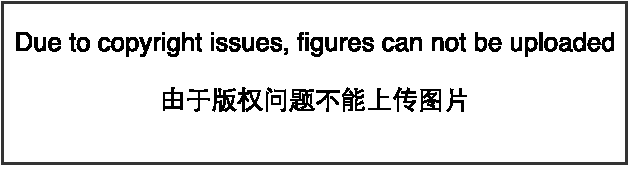
\includegraphics{figure.pdf}}
\else
\begin{tabular}{ccccccc}
\includegraphics[width=0.1\textwidth]{Chapter15/figures/man_with_glasses} &
- &
\includegraphics[width=0.1\textwidth]{Chapter15/figures/man_without_glasses} &
+ &
\includegraphics[width=0.1\textwidth]{Chapter15/figures/woman_without_glasses} &
= &
\includegraphics[width=0.3\textwidth]{Chapter15/figures/woman_with_glasses}
\end{tabular}
\fi
\caption{\gls{generative_model}学到了\gls{distributed_representation},能够从戴眼镜的概念中区分性别的概念。
如果我们从一个戴眼镜的男人的概念表示向量开始,然后减去一个没戴眼镜的男人的概念表示向量,最后加上一个没戴眼镜的女人的概念表示向量,那么我们会得到一个戴眼镜的女人的概念表示向量。
\gls{generative_model}将所有这些表示向量正确地解码为可被识别为正确类别的图像。
图片转载许可自\cite{radford2015unsupervised}。
}
\label{fig:chap15_generative_glasses}
\end{figure}

% 542 end

\section{得益于深度的指数增益}
\label{sec:exponential_gains_from_depth}
我们已经在\secref{sec:universal_approximation_properties_and_depth}中看到,\gls{MLP}是\gls{universal_approximator},相比于浅层网络,一些函数能够用指数级小的\gls{deep_network}表示。
缩小模型规模能够提高统计效率。
在本节中,我们描述如何将类似结果更一般地应用于其他具有分布式隐藏表示的模型。

% 543 mid

在\secref{sec:distributed_representation}中,我们看到了一个\gls{generative_model}的示例,能够学习人脸图像的\gls{underlying}\gls{explanatory_factor},包括性别以及是否佩戴眼镜。
完成这个任务的\gls{generative_model}是基于一个\gls{DNN}的。
浅层网络例如线性网络不能学习出这些抽象\gls{explanatory_factor}和图像像素之间的复杂关系。
在这个任务和其他\glssymbol{AI}任务中,这些因子几乎彼此独立地被抽取,但仍然对应到有意义输入的因素,很有可能是高度抽象的,并且和输入呈高度非线性的关系。
我们认为这需要\emph{深度}\gls{distributed_representation},需要许多非线性组合来获得较高级的特征(被视为输入的函数)或因子(被视为生成原因)。

% 543 mid

在许多不同\gls{setting}中已经证明,
非线性和重用特征层次结构的组合来组织计算,可以使\gls{distributed_representation}获得指数级加速之外,还可以获得统计效率的指数级提升。
许多种类的只有一个\gls{hidden_layer}的网络(例如,具有饱和非线性,布尔门,和/积,或\glssymbol{RBF}单元的网络)都可以被视为\gls{universal_approximator}。
在给定足够多\gls{hidden_unit}的情况下,这个模型族是一个\gls{universal_approximator},可以在任意非零允错级别近似一大类函数(包括所有连续函数)。
然而,\gls{hidden_unit}所需的数量可能会非常大。
关于深层架构表达能力的理论结果表明,有些函数族可以高效地通过深度$k$层的网络架构表示,但是深度不够(深度为2或$k-1$)时会需要指数级(相对于输入大小而言)的\gls{hidden_unit}。

% -- 543 end

% 544 head

在\secref{sec:universal_approximation_properties_and_depth}中,我们看到确定性\gls{feedforward_network}是函数的\gls{universal_approximator}。
许多具有单个\gls{hidden_layer}(\gls{latent_variable})的\gls{structured_probabilistic_models}(包括\gls{RBM},\gls{DBN})是概率分布的\gls{universal_approximator}~\citep{LeRoux-Bengio-2007-TR,Montufar-2011,Montufar-et-al-NIPS2014,Krause-et-al-ICML2013}。

% 544 mid

在\secref{sec:universal_approximation_properties_and_depth}中,我们看到足够深的\gls{feedforward_network}会比深度不够的网络具有指数级优势。
这样的结果也能从诸如概率模型的其他模型中获得。
\firstall{sum_product_network}%,\glssymbol{sum_product_network}
~\citep{Poon+Domingos-2011}是这样的一种概率模型。
这些模型使用多项式回路来计算一组\gls{RV}的\gls{PD}。
\cite{Delalleau+Bengio-2011-small}表明存在一种\gls{PD},对\glssymbol{sum_product_network}的最小深度有要求,以避免模型规模呈指数级增长。
后来,\cite{Martens+Medabalimi-arxiv2014}表明,任意两个有限深度的\glssymbol{sum_product_network}之间都会存在显著差异,并且一些使\glssymbol{sum_product_network}易于处理的约束可能会限制其表示能力。

% 544 mid

另一个有趣的进展是,一系列和\gls{convolutional_net}相关的\gls{deep_circuit}族表达能力的理论结果,即使让\gls{shadow_circuit}只去近似\gls{deep_circuit}计算的函数,也能突出反映\gls{deep_circuit}的指数级优势~\citep{Cohen-et-al-arXiv2015}。
相比之下,以前的理论工作只研究了\gls{shadow_circuit}必须精确复制特定函数的情况。

% 544 mid

\section{提供发现潜在原因的线索}
\label{sec:providing_clues_to_discover_underlying_causes}

% 544 end

我们回到最初的问题之一来结束本章:什么原因能够使一个表示比另一个表示更好?
首先在\secref{sec:semi_supervised_disentangling_of_causal_factors}中介绍的一个答案是,一个理想的表示能够区分生成数据变化的\gls{underlying}\gls{causal_factor},特别是那些与我们的应用相关的因素。
\gls{representation_learning}的大多数策略都会引入一些有助于学习\gls{underlying}\gls{factors_of_variation}的线索。
这些线索可以帮助\gls{learner}将这些观察到的因素与其他因素分开。
\gls{supervised_learning}提供了非常强的线索:每个观察向量$\Vx$的\gls{label}$\Vy$,它通常直接指定了至少一个\gls{factors_of_variation}。
更一般地,为了利用丰富的\gls{unlabeled}数据,\gls{representation_learning}会使用关于\gls{underlying}因素的其他不太直接的提示。
这些提示包含一些我们(学习算法的设计者)为了引导\gls{learner}而强加的隐式先验信息。
诸如\gls{no_free_lunch_theorem}的这些结果表明,\gls{regularization}策略对于获得良好\gls{generalization}是很有必要的。
当不可能找到一个普遍良好的\gls{regularization}策略时,\gls{DL}的一个目标是找到一套相当通用的\gls{regularization}策略,使其能够适用于各种各样的\glssymbol{AI}任务(类似于人和动物能够解决的任务)。

% 545 head

在此,我们提供了一些通用\gls{regularization}策略的列表。
该列表显然是不详尽的,但是给出了一些学习算法是如何发现对应\gls{underlying}因素的特征的具体示例。
该列表在\cite{Bengio-Courville-Vincent-TPAMI-2012}的第3.1节中提出,这里进行了部分拓展。
\begin{itemize}
	\item \emph{平滑}:假设对于单位$\Vd$和小量$\epsilon$有$f(\Vx + \epsilon \Vd) \approx f(\Vx)$。
	这个假设允许\gls{learner}从训练样本\gls{generalize}到输入空间中附近的点。
	许多\gls{ML}算法都利用了这个想法,但它不能克服\gls{curse_of_dimensionality}难题。


	\item \emph{线性}:很多学习算法假定一些变量之间的关系是线性的。
	这使得算法能够预测远离观测数据的点,但有时可能会导致一些极端的预测。
	大多数简单的学习算法不会做平滑假设,而会做线性假设。
	这些假设实际上是不同的,具有很大权重的线性函数在高维空间中可能不是非常平滑的。
	参看\cite{Goodfellow-2015-adversarial}了解关于线性假设局限性的进一步讨论。

% 545 mid

	\item \emph{多个\gls{explanatory_factor}}:许多\gls{representation_learning}算法受以下假设的启发,数据是由多个\gls{underlying}\gls{explanatory_factor}生成的,并且给定每一个因子的状态,大多数任务都能轻易解决。
	\secref{sec:semi_supervised_disentangling_of_causal_factors}描述了这种观点如何通过\gls{representation_learning}来启发\gls{semi_supervised_learning}的。
	学习$p(\Vx)$的结构要求学习出一些对建模$p(\Vy\mid\Vx)$同样有用的特征,因为它们都涉及到相同的\gls{underlying}\gls{explanatory_factor}。
	\secref{sec:distributed_representation}介绍了这种观点如何启发\gls{distributed_representation}的使用,表示空间中\gls{separate}方向对应着\gls{separate}\gls{factors_of_variation}。


	\item \emph{\gls{causal_factor}}:该模型认为\gls{learned}表示所描述的\gls{factors_of_variation}是观察数据$\Vx$的成因,而并非反过来。
	正如\secref{sec:semi_supervised_disentangling_of_causal_factors}中讨论的,这对于\gls{semi_supervised_learning}是有利的,当\gls{underlying_cause}上的分布发生改变,或者我们应用模型到一个新的任务上时,\gls{learned}的模型都会更加鲁棒。

% -- 546 head

	\item \emph{深度,或者\gls{explanatory_factor}的层次组织}:高级抽象概念能够通过将简单概念层次化来定义。
	从另一个角度来看,深度架构表达了我们认为任务应该由多个程序步骤完成的观念,其中每一个步骤回溯到先前步骤处理之后的输出。


	\item \emph{任务间共享因素}:
	当多个对应到不同变量$\RSy_i$的任务共享相同的输入$\RVx$时,或者当每个任务关联到全局输入$\RVx$的子集或者函数$f^{(i)}(\RVx)$时,我们会假设每个变量$\RSy_i$关联到来自相关因素$\RVh$公共池的不同子集。
	因为这些子集有重叠,所以通过共享的中间表示$ P(\RVh \mid \RVx)$来学习所有的$P(\RSy_i \mid \RVx)$能够使任务间共享统计强度。

% -- 546 mid

	\item \emph{\gls{manifold}}:概率质量集中,并且集中区域是局部连通的,且占据很小的体积。
	在连续情况下,这些区域可以用比数据所在原始空间低很多维的低维\gls{manifold}来近似。
	很多\gls{ML}算法只在这些\gls{manifold}上有效\citep{Goodfellow-2015-adversarial}。
	一些\gls{ML}算法,特别是\gls{AE},会试图显式地学习\gls{manifold}的结构。


	\item \emph{自然聚类}:很多\gls{ML}算法假设输入空间中每个连通\gls{manifold}可以被分配一个单独的类。
	数据分布在许多个不连通的\gls{manifold}上,但相同\gls{manifold}上数据的类别是相同的。
	这个假设激励了各种学习算法,包括\gls{tangent_propagation}、\gls{double_backprop}、\gls{manifold_tangent_classifier}和\gls{adversarial_training}。


	\item \emph{时间和空间相干性}:\gls{SFA}和相关的算法假设,最重要的\gls{explanatory_factor}随时间变化很缓慢,或者至少假设预测真实的\gls{underlying}\gls{explanatory_factor}比预测诸如像素值这类原始观察会更容易些。
	读者可以参考\secref{sec:slow_feature_analysis},进一步了解这个方法。


	\item \emph{稀疏性}:假设大部分特征和大部分输入不相关,如在表示猫的图像时,没有必要使用象鼻的特征。
	因此,我们可以强加一个先验,任何可以解释为``存在''或``不存在''的特征在大多数时间都是不存在的。

% -- 547 head --

	\item \emph{简化因子\gls{dependency}}:在良好的高级表示中,因子会通过简单的\gls{dependency}相互关联。
	最简单的可能是边缘独立,即$P(\RVh) = \prod_i P(\RVh_i)$。
	但是线性\gls{dependency}或浅层\gls{AE}所能表示的\gls{dependency}关系也是合理的假设。
	这可以从许多物理定律中看出来,并且假设在\gls{learned}表示的顶层插入线性预测器或\gls{factorized}先验。
\end{itemize}


\gls{representation_learning}的概念将许多\gls{DL}形式联系在了一起。
\gls{feedforward_network}和\gls{recurrent_network},\gls{AE}和深度概率模型都在学习和使用表示。
学习最佳表示仍然是一个令人兴奋的研究方向。

% -- 547 --
